\documentclass[14pt, a4paper]{article}
\usepackage{minitoc}
\usepackage[left=3.00cm, right=2.5cm, top=2.00cm, bottom=2.00cm]{geometry}
\usepackage{amsmath}
\usepackage{amssymb}
\usepackage{amsthm}
\usepackage{mathtools}
\usepackage{graphicx}
%\usepackage{algpseudocode}
%\usepackage{algorithm}
\usepackage[ruled,vlined,linesnumbered]{algorithm2e}
\usepackage{blindtext}
\usepackage{setspace}
\usepackage[utf8]{inputenc}
\usepackage[utf8]{vietnam}
\usepackage[center]{caption}
\usepackage[shortlabels]{enumitem}
\usepackage{fancyhdr} % header, footer
\usepackage{hyperref} % loại bỏ border với mục lục và công thức
\usepackage[nonumberlist, nopostdot, nogroupskip]{glossaries}
\usepackage{glossary-superragged}
\usepackage{tikz,tkz-tab}
\usepackage{pythonhighlight}
\setglossarystyle{superraggedheaderborder}
\pagestyle{fancy}
%\usepackage[style=numeric,sortcites]{biblatex}
%\addbibresource{ref.bib}
%\usepackage[numbers]{natbib}
\usepackage{indentfirst}
\usepackage[natbib,backend=biber,style=ieee, sorting=ynt]{biblatex}
\bibliography{ref.bib}

\graphicspath{{./figures/}}

\fancyhf{}
%\rhead{\textbf{Môn học: Các phương pháp thống kê hiện đại trong nghiên cứu Xã hội học}}
\lhead{\textbf{GVHD: TS. Trịnh Quốc Anh}}
\rfoot{\thepage}
\lfoot{\textbf{Học viên thực hiện: Nguyễn Chí Thanh - 21007925}}
\renewcommand{\headrulewidth}{0.4pt}
\renewcommand{\footrulewidth}{0.4pt}
%
%\numberwithin{equation}{section}
%\numberwithin{algorithm}{section}
%\numberwithin{figure}{section}
%
%\setlength{\parindent}{0.5cm}
%
%\setcounter{secnumdepth}{3} % Cho phép subsubsection trong report
%\setcounter{tocdepth}{3} % Chèn subsubsection vào bảng mục lục

%\newtheorem{dl}{Định lý}
%\newtheorem{md}{Mệnh đề}
%\newtheorem{bd}{Bổ đề}
%\newtheorem{dn}{Định nghĩa}
%\newtheorem{hq}{Hệ quả}

%\newtheorem{baitap}{Bài tập}
%\newtheorem*{loigiai}{Lời giải}

%\numberwithin{dl}{section}
%\numberwithin{md}{section}
%\numberwithin{bd}{section}
%\numberwithin{dn}{section}
%\numberwithin{hq}{section}

\setlength{\parindent}{0cm}

\newtheorem{dl}{Định lý}
\newtheoremstyle{sltheorem}
{}                % Space above
{}                % Space below
{\normalfont}        % Theorem body font % (default is "\upshape")
{}                % Indent amount
{\bfseries}       % Theorem head font % (default is \mdseries)
{.}               % Punctuation after theorem head % default: no punctuation
{ }               % Space after theorem head
{}                % Theorem head spec
\theoremstyle{sltheorem}
\newtheorem{baitap}{Bài tập}
\newtheoremstyle{soltheorem}
{}                % Space above
{}                % Space below
{\normalfont}        % Theorem body font % (default is "\upshape")
{}                % Indent amount
{\bfseries}       % Theorem head font % (default is \mdseries)
{.}               % Punctuation after theorem head % default: no punctuation
{\newline}               % Space after theorem head
{}                % Theorem head spec
\theoremstyle{soltheorem}
\newtheorem*{loigiai}{Lời giải}

\onehalfspacing


\begin{document}
\begin{titlepage}

    \newcommand{\HRule}{\rule{\linewidth}{0.5mm}} % Defines a new command for the horizontal lines, change thickness here

    \center % Center everything on the page

    %----------------------------------------------------------------------------------------
    %	HEADING SECTIONS
    %----------------------------------------------------------------------------------------
    \textsc{\LARGE Đại học Quốc Gia Hà Nội}\\[0.5cm]
    \textsc{\LARGE Trường đại học Khoa học tự nhiên}\\[0.5cm] % Name of your university/college
    \textsc{\LARGE Khoa Toán - Cơ - Tin học}\\[0.5cm]

    
\includegraphics[scale=0.2]{HUS-logo.jpg}\\[0.5cm]

    \textsc{\Large Chuyên ngành: Khoa học dữ liệu}\\[0.5cm] % Major heading such as course name


    %----------------------------------------------------------------------------------------
    %	TITLE SECTION
    %----------------------------------------------------------------------------------------

    \HRule \\[0.4cm]
    { \huge \bfseries Bài tập môn học}\\[0.4cm] % Title of your document
    \HRule \\[1.5cm]

    \textsc{\Large Môn học: Các phương pháp thống kê hiện đại \\ trong nghiên cứu Xã hội học}\\[1cm] % Minor heading such as course title


    \textsc{\Large Bài tập 1}\\[1cm]


    %----------------------------------------------------------------------------------------
    %	AUTHOR SECTION
    %----------------------------------------------------------------------------------------
    \begin{minipage}{0.4\textwidth}
        \begin{flushleft} \large
        \emph{Giảng viên hướng dẫn:} \\
        TS. Trịnh Quốc Anh % Supervisor's Name
        \end{flushleft}
    \end{minipage}\\[0.5cm]

    \begin{minipage}{0.4\textwidth}
    \begin{flushleft} \large
    \emph{Học viên thực hiện:}\\
    Nguyễn Chí Thanh \\
    MSHV: 21007925 \\ % Your name
    Lớp: Khoa học dữ liệu - K4
    \end{flushleft}
    \end{minipage}


    % If you don't want a supervisor, uncomment the two lines below and remove the section above
    %\Large \emph{Author:}\\
    %John \textsc{Smith}\\[3cm] % Your name

    %----------------------------------------------------------------------------------------
    %	DATE SECTION
    %----------------------------------------------------------------------------------------

    % I don't want day because it is English
    % {\large \today}\\[2cm] % Date, change the \today to a set date if you want to be precise

    %----------------------------------------------------------------------------------------
    %	LOGO SECTION
    %----------------------------------------------------------------------------------------

    %\includegraphics{logo/rsz_3logo-khtn.png}\\[1cm] % Include a department/university logo - this will require the graphicx package

    %----------------------------------------------------------------------------------------

    \vfill % Fill the rest of the page with whitespace

\end{titlepage}

\nocite{*}

\newpage

\begin{baitap}
    Hãy tóm tắt về nghiên cứu "Hút thuốc khi mang thai và sức khoẻ trẻ sơ sinh":
    \begin{itemize}
        \item Vấn đề/câu hỏi cần nghiên cứu.
        \item Dữ liệu dùng để nghiên cứu.
        \item Cơ sở và phương pháp nghiên cứu
    \end{itemize}
\end{baitap}

\begin{loigiai}
    Hãy tóm tắt về nghiên cứu "Hút thuốc khi mang thai và sức khoẻ trẻ sơ sinh":
    \begin{itemize}
        \item Vấn đề/câu hỏi cần nghiên cứu: Sự khác biệt giữa cân nặng, sức khỏe và tỷ lệ tử vong của trẻ sơ sinh được sinh bởi người mẹ có hút thuốc trong thời gian mang thai hoặc người mẹ không hút thuốc trong thời gian mang thai.
        \item Dữ liệu dùng để nghiên cứu:
        Dữ liệu được sử dụng cho lab là một tập con của một tập dữ liệu nghiên cứu lớn hơn nhiều - Nghiên cứu về sức khỏe và sự phát triển trẻ em \cite{yerushalmy1964mother}. 
        Toàn bộ tập dữ liệu ghi lại tất cả các trường hợp mang thai xảy ra từ năm 1960 đến 1967 ở những người phụ nữ trong Kaiser Foundation Health Plan  tại Oakland, California, Kaiser Foundation Plan là một chương trình chăm sóc y tế trả trước. 
        Những người phụ nữ trong nghiên cứu đều là những người đã đăng ký tham gia vào Kaiser Plan và được chăm sóc trước khi sinh ở khu vực San Francisco - East Bay và đã sinh tại bất kỳ bệnh viện nào của Kaiser ở Bắc California.

        Khi nghiên cứu 15000 gia đình tham gia vào nghiên cứu \cite{yerushalmy1964mother} đã tuyên bố rằng:

        \begin{itemize}
            \item Những phụ nữ tham gia chương trình chăm sóc y tế tại Kaiser tương đối sớm trong thai kỳ.
            Hai phần ba trong báo cáo là vào 3 tháng đầu tiên, gần một phần hai khi đang mang thai 2 tháng hoặc ít hơn. 
            Các gia đình tham gia nghiên cứu nằm trong đa dạng các đặc điểm kinh tế, xã hội và giao dục. 
            Gần hai phần ba là người da trắng, một phần năm là người da màu, 3 đến 4 \% là người phương Đông, và còn lại các các chủng tộc khác và các hôn nhân hỗn hợp màu da. Khoảng 30 \% các ông chồng làm nghề chuyên nghiệp. 
            Một lượng lớn là các thành viên của các hiệp hội khác nhau. Gần 10 \% đang làm việc tại Đại học California Berkeley trong các vị trí học thuật hoặc hành chính, và 20 phần trăm là trong cơ quan chính phủ. 
            Trình độ học vấn cao hơn chút so với mặt bằng chung bang California cũng như thu nhập trung bình. 
            Vì vậy đối tương nghiên cứu nói chung không phải là điển hình của dân số có việc làm. Những người tham gia thiếu phân khúc rất nghèo hoặc rất giàu vì những những nhóm này không có khả năng đại diện trong một chương trình y tế trả trước.
            \item Khi sinh ra, các phép đo sẽ được thực hiện trên các em bé. 
            Bao gồm chiều dài, cân nặng và chu vi vòng đầu của em bé. 
            Được cung cấp ở đây là một tập con của thông tin thu thập từ 1236 em bé - những bé trai được sinh ra trong một năm của nghiên cứu đã sống ít nhất 28 ngày và là trẻ được sinh một (tức là không phải là một trong các cặp song sinh hoặc sinh ba). 
            Thông tin có cho mỗi em bé là cân nặng khi sinh và người mẹ có hút thuốc khi mang thai hay không.
        \end{itemize}
        \item Cơ sở và phương pháp nghiên cứu:
        \begin{itemize}
            \item Tổng hợp hai phân phối của khối lượng khi sinh của trẻ em với mẹ có hút thuốc hoặc không trong thời gian thai kỳ.
            \item Sử dụng các phương pháp trực quan để so sánh hai phân phối cân nặng khi sinh.
            \item So sánh tần suất hoặc tỷ lệ trẻ sơ sinh bị nhẹ cân của hai nhóm. Các ước lượng có độ tin cậy thế nào? Làm thế nào tỷ lệ trẻ nhẹ cân thay đổi nếu có thêm hoặc ít trẻ hơn được xếp vào nhóm trẻ nhẹ cân.
            \item Đánh giá mức độ quan trọng sự khác biệt trong các cách so sánh: số liệu, đồ thị, biểu đồ, tỷ lệ.
        \end{itemize}
    \end{itemize}
\end{loigiai}


\begin{baitap}
    Trả lời các câu hỏi 1 - 12, của quyển sách \cite{nolan2001stat}, trang 21 - 23
\end{baitap}

\begin{loigiai}
    Trả lời các câu hỏi 1 - 12, của quyển sách \cite{nolan2001stat}, trang 21 - 23
    \begin{enumerate}[wide, labelwidth=!, labelindent=0pt,label=\textbf{\arabic*}.]
        \item Sử dụng bảng \ref{tb:1.3} để ước lượng các phân vị phần tư của phân phối của số điếu thuốc đượt hút một ngày của các bà mẹ hút trong thời gian thai kỳ từ CHDS.

            \begin{table}[h!]
                \begin{center}
                    \begin{tabular}{|c|c|}
                        \hline
                        \textbf{Số điếu thuốc được hút} & \textbf{Tỷ lệ trong số người hút thuốc} \\  
                        \hline
                        0--5 & 16\% \\  
                        5--10 & 25\% \\  
                        10--15 & 14\% \\  
                        15--20 & 4\% \\  
                        20--30 & 32\% \\  
                        30--40 & 5\% \\  
                        40--60 & 4\% \\  
                        \hline
                        Tổng cộng & 100 \% \\
                        \hline
                    \end{tabular}
                \end{center}
                \caption{Bảng tần suất của số điếu thuốc được hút trong một ngày của 484 bà mẹ trong tập CHDS có hút thuốc trong thời gian thai kỳ,
                tỷ lệ phần trăm được làm tròn đến số nguyên gần nhất}
                \label{tb:1.3}
            \end{table}
        
        Ta có:
        \begin{equation*}
            \begin{aligned}
                &Q_1 = 5 + \dfrac{10 - 5}{25} \times (25 - 16) = 6.80 \\
                &Q_2 = 10 + \dfrac{15 - 10}{14} \times (50 - 41) = 13.21 \\
                &Q_3 = 20 + \dfrac{30 - 20}{32} \times (75 - 59) = 25
            \end{aligned}
        \end{equation*}

        \item Hợp bốn nhóm cuối trong bảng \ref{tb:1.3} thành một nhóm của phân phối số điếu thuốc đượt hút một ngày của các bà mẹ hút trong thời gian thai kỳ từ CHDS.
        Xây dựng histogram mới từ bảng thu được. Hình dạng thay đổi như nào so với histogram cũ?

        Ta có bảng phân phối mới sau khi hợp bốn nhóm cuối trong bảng \ref{tb:1.3}:

        \begin{table}[h!]
            \begin{center}
                \begin{tabular}{|c|c|}
                    \hline
                    \textbf{Số điếu thuốc được hút} & \textbf{Tỷ lệ trong số người hút thuốc} \\  
                    \hline
                    0--5 & 16\% \\  
                    5--10 & 25\% \\  
                    10--15 & 14\% \\  
                    15--60 & 45\% \\  
                    \hline
                    Tổng cộng & 100 \% \\
                    \hline
                \end{tabular}
            \end{center}
            \caption{Bản tần suất của số điếu thuốc được hút trong một ngày của 484 bà mẹ trong tập CHDS có hút thuốc trong thời gian thai kỳ,
            tỷ lệ phần trăm được làm tròn đến số nguyên gần nhất}
        \end{table}

        Ta sử dụng code để vẽ histogram mới:

        \begin{python}
import numpy as np
import matplotlib.pyplot as plt
            
            
lower = np.array([0, 5, 10, 15])
upper = np.array([5, 10, 15, 60])
            
percent = np.array([16, 25, 14, 45])
            
plt.bar(lower, percent/(upper-lower), width=upper - lower, ec="k", align="edge")
plt.xticks(lower.tolist() + [upper.tolist()[-1]], rotation=45)
plt.xlabel("Number of cigarettes (per day)")
plt.ylabel("Percent per cigarette")
plt.grid()
plt.show()
        \end{python}

        \begin{figure}[h!]
            \centering
            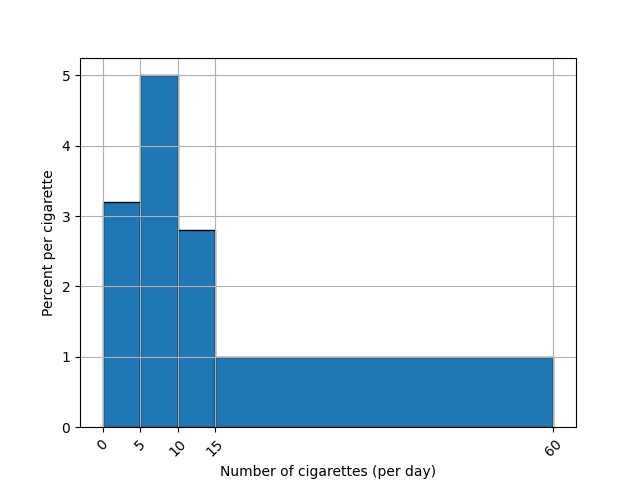
\includegraphics[scale=0.8]{2.png}
            \caption{histogram mới sau khi hợp bốn nhóm cuối bảng \ref{tb:1.3}}
        \end{figure}

        \item Ta xét histogram của tuổi của những người cha trong tập CHDS (hình \ref{fig:1.14}). Cột tương ứng với khoảng tuổi từ 35 đến 40 tuổi bị mất. Tìm chiều cao của cột này.
        \begin{figure}[h!]
            \centering
            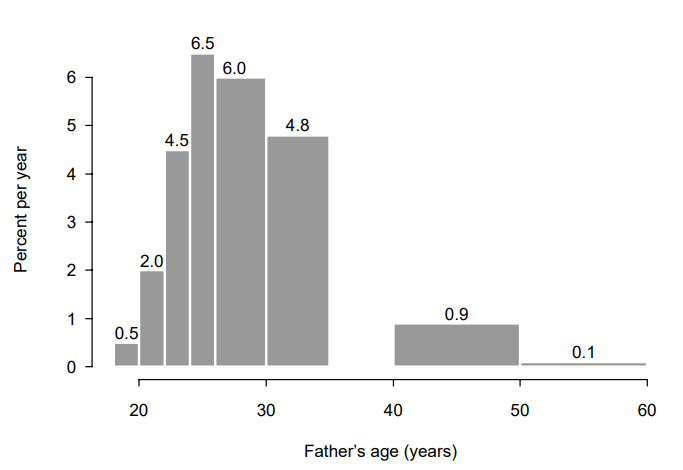
\includegraphics[scale=0.8]{1.14.png}
            \caption{Tuổi của những người cha (năm)}
            \label{fig:1.14}
        \end{figure}

        Ta đặt chiều cao của cột tương ứng với khoảng 35 - 40 tuổi là $x$:

        \begin{equation*}
            \begin{aligned}
                &0.5 \times 2 + 2.0 \times 2 + 4.5 \times 2 + 6.5 \times 2 + 6.0 \times 4 + 4.8 \times 5 + x \times 5 + 0.9 \times 10 + 0.1\times 10 = 100 \\
                &\Rightarrow x = \dfrac{100 - (0.5 \times 2 + 2.0 \times 2 + 4.5 \times 2 + 6.5 \times 2 + 6.0 \times 4 + 4.8 \times 5 + 0.9 \times 10 + 0.1\times 10)}{5} = \dfrac{100-85}{5}=3 \%
            \end{aligned}
        \end{equation*}

        Vậy chiều cao của cột tương ứng với khoảng 35 - 40 tuổi là 3 \%

        \item Ta xét quantile plot của chiều cao và cân nặng của những người cha trong CHDS (hình \ref{fig:1.15}). Hãy miêu tả hình dạng của các phân phối trên.
        \begin{figure}[h!]
            \centering
            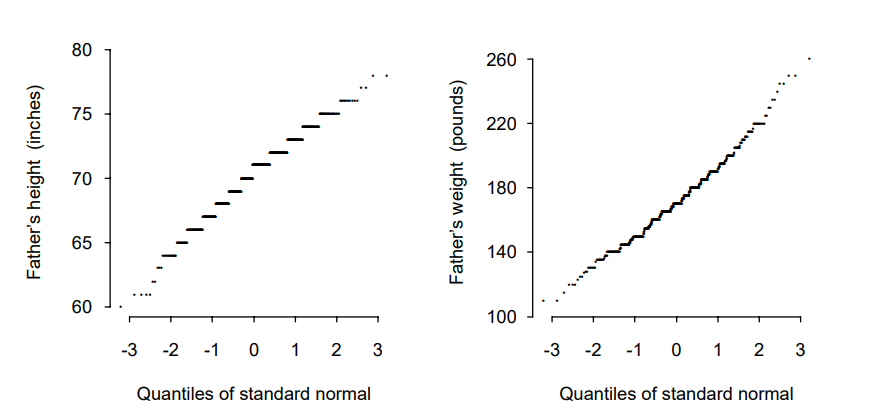
\includegraphics[scale=0.7]{1.15.png}
            \caption{Đồ thị quantile của chiều cao của những người cha (bên trái) và cân nặng (bên phải) trong tập CHDS.}
            \label{fig:1.15}
        \end{figure}

        Đồ thị quantile của chiều cao của những người cha cho thấy chiều cao được đo là một đại lượng rời rạc.
        Ta nhận thấy các điểm gần như nằm trên một đường thẳng cho thấy phân phối chiều cao của những người cha xấp xỉ phân phối chuẩn.
        
        \begin{figure}[h!]
            \centering
            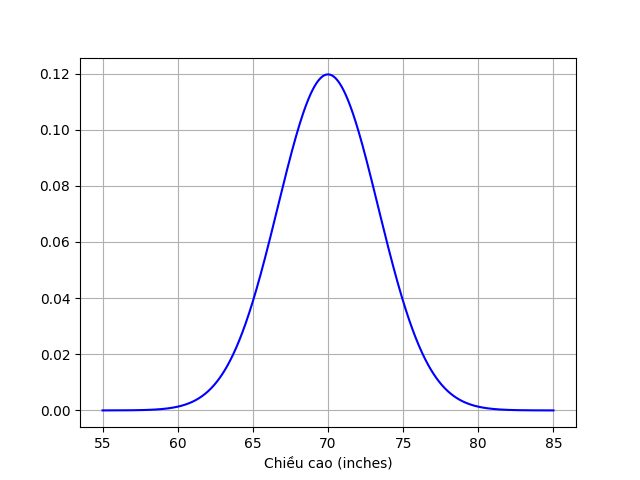
\includegraphics[scale=0.7]{4.1.png}
            \caption{Đồ thị hàm mật độ lý thuyết chiều cao của những người cha}
        \end{figure}

        Đồ thị quantile cân nặng của người cha cho thấy các điểm nằm khá sát trên một đường thẳng nên phân phối có dạng xấp xỉ phân phối chuẩn và phân phối khá đối xứng nhưng có khá ít điểm rơi vào khoảng biên và đa số các điểm tập trung ở khu vực trung nên cho ta thấy phân phối có hai bên đuôi khá nhẹ.
        
        \begin{figure}[h!]
            \centering
            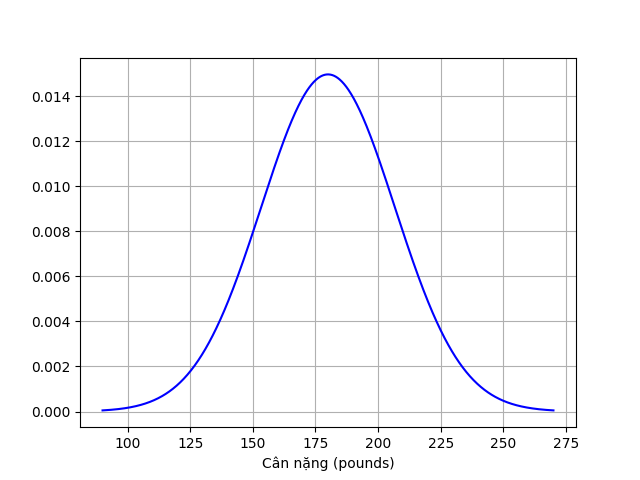
\includegraphics[scale=0.7]{4.2.png}
            \caption{Đồ thị hàm mật độ lý thuyết cân nặng của những người cha}
        \end{figure}

        \item Theo các phân vị 0.05, 0.1, \dots, 0.95 cho thời gian thai kỳ của em bé trong tập CHDS.
        Miêu tả hình dạng của phân phối của thời gian thai kỳ so với phân phối đều.
        252, 262, 267, 270, 272, 274, 276, 277, 278, 280, 281, 283, 284, 286, 288, 290, 292, 296, 302.
        
        Ta sử dụng đoạn code sau để vẽ đồ thị quantile của số liệu trên.

        \begin{python}
import numpy as np 
import pylab 
import scipy.stats as stats
import matplotlib.pyplot as plt
            
measurements = np.array([252, 262, 267, 270, 272, 274, 276, 277, 278, 280, 281, 283, 284, 286, 288, 290, 292, 296, 302])
quantiles = np.arange(1, measurements.shape[0] + 1) / (measurements.shape[0] + 1)
print(quantiles)
#plt.scatter(quantiles, measurements)
#plt.grid()
#plt.show()
stats.probplot(measurements, dist="uniform", plot=pylab)
pylab.title("Quantile plot")
pylab.xlabel("Quantiles of uniform")
pylab.ylabel("Gestational age")
pylab.grid()
pylab.show()
        \end{python}

        \begin{figure}[h!]
            \centering
            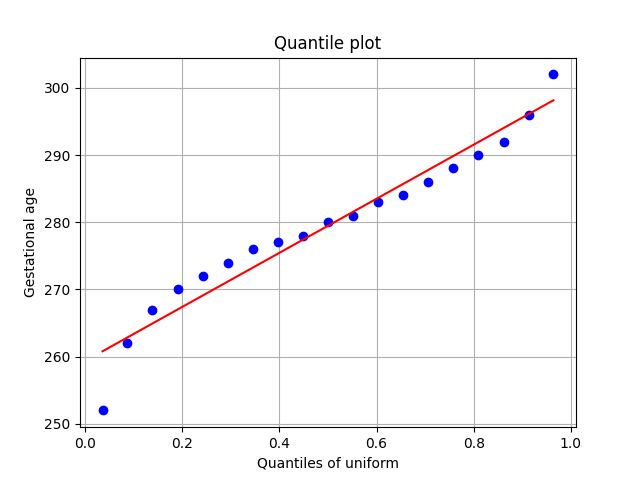
\includegraphics[scale=0.7]{5.png}
            \caption{Đồ thị quantile tương ứng với phân phối dữ liệu thời gian thai kỳ của em bé.}
        \end{figure}

        Từ đồ thị quantile ta nhận thấy phân phối thời gian thai kỳ của em bé có đuôi bên trái và bên phải dài hơn so với phân phối đều.

        \item Sử dụng xấp xỉ phân phối chuẩn ước lượng tỷ lệ của người mẹ trong tập CHDS có chiều cao từ 62 đến 64 inches đến nửa inch gần nhất (nằm giữa 61.5 và 64.5 inch).
        Chiều cao trung bình là 64 inch và độ lệch tiêu chuẩn SD là 2.5 inches.

        Ta gọi $X$ (inches) là chiều cao của các bà mẹ.
        \begin{equation*}
            X \sim \mathcal{N} (64; 2.5^2)
        \end{equation*}

        Ta cần tính $P(61.5 \leq X \leq 64.5)$:

        \begin{equation*}
            \begin{aligned}
                P (61.5 \leq X \leq 64.5) &= P \Big( \dfrac{61.5 - 64}{2.5} \leq \dfrac{Z - 64}{2.5} \leq \dfrac{64.5 - 64}{2.5} \Big) \\
                &= P (-1 \leq Z \leq 0.2) \\
                &= \Phi (0.2) - \Phi (-1) \\
                &= \Phi (0.2) - (1 - \Phi(1)) \\
                &= \Phi(0.2) + \Phi(1) - 1 \\
                &= 0.57926 + 0.84134 - 1 \\
                &= 0.4206
            \end{aligned}
        \end{equation*}

        \item Hai từ cần điền vào chỗ trống là:
        Vị trí thứ nhất: 2180
        Vị trí thứ hai: 2.64

        \item Ta giả sử có 100 quan sát từ phân phối chuẩn tắc.
        Tỷ lệ trong số các quan sát này mà ta kỳ vọng nằm ngoài whisker của một đồ thị whisker and box?


        Đối với phân phối chuẩn tắc ta có $z_{0.25}=-0.6745$ và $z_{0.75}=0.6745$ hay $Q_1=-0.6745$ và $Q_3=0.6745$.
        Vậy $IQR=Q_3 - Q_1 = 0.6745 - (-0.6745)=1.349$.

        Xác suất để một quan sát nằm ngoài whisker là:

        \begin{equation*}
            \begin{aligned}
                P (Z < Q_1 - 1.5 \times IQR \cup Z > Q_3 + 1.5 \times IQR) &= P (Z < Q_1 - 1.5 \times IQR) + P (Z > Q_3 + 1.5 \times IQR) \\
                &= P(Z < -0.6745 - 1.5 \times 1.349) + P (Z > 0.6745 + 1.5 \times 1.349) \\
                &= P(Z < -2.648) + P (Z > 2.698) \\
                &= \Phi(-2.698) + (1 - \Phi(2.698)) \\
                &= (1 - \Phi(2.698)) + (1 - \Phi(2.698)) \\
                &= 2 \times (1 - \Phi(2.698)) \\
                &= 0.00698 = 0.698 \%
            \end{aligned}
        \end{equation*}

        Như vậy tỷ lệ số quan sát nằm ngoài whisker của một đồ thị whisker and box là 0.698 \%.
        Và như vậy chỉ có khoảng 1 quan sát nằm ngoài whisker của một đồ thị whisker and box.

        \item Tạo một bảng của tình trạng hôn nhân cho biết tỷ lệ người hút thuốc và không hút thuốc trong từng nhóm tình trạng hôn nhân của các bà mẹ trong nghiên cứu Missouri (hình \ref{fig:Table1.16}).
        \begin{figure}[h!]
            \centering
            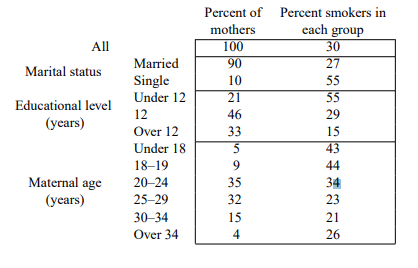
\includegraphics[scale=0.8]{Table1.6.png}
            \caption{Tỷ lệ người mẹ hút thuốc theo từng nhóm đặc trưng theo tình trạng hôn nhân, học vấn và tuổi}
            \label{fig:Table1.16}
        \end{figure}

        \begin{table}[h!]
            \begin{center}
                \begin{tabular}{|c|c|c|}
                    \hline
                    Tình trạng hôn nhân& Tỷ lệ người hút thuốc & Tỷ lệ người không hút thuốc \\  
                    \hline
                    Đã kết hôn & 27 \% & 73 \% \\
                    \hline
                    Độc thân & 55 \% & 45 \% \\
                    \hline
                \end{tabular}
            \end{center}
            \caption{Tỷ lệ các bà mẹ hút thuốc trong thời kỳ mang thai theo tình trạng hôn nhân trong nghiên cứu Missouri}
            \label{tb:Marital-status}
        \end{table}
        Bảng của tình trạng hôn nhân cho biết tỷ lệ người hút thuốc và không hút thuốc trong từng nhóm tình trạng hôn nhân của các bà mẹ trong nghiên cứu Missouri được thể hiện ở bảng \ref{tb:Marital-status}

        \item Tạo một biểu đồ cột chồng thể hiện tỷ lệ về các cấp độ học vấn cho cả các bà mẹ hút thuốc và không hút thuốc trong thời gian thai kỳ trong nghiên cứu Missouri (hình \ref{fig:Table1.16})
        
        Ta gọi $A$ là sự kiện một bà mẹ ở nhóm trình độ dưới lớp 12.
        Ta gọi $B$ là sự kiện một bà mẹ ở nhóm trình độ lớp 12.
        Ta gọi $C$ là sự kiện một bà mẹ ở nhóm trình độ trên lớp 12.

        Ta gọi $Y$ là sự kiện một bà mẹ hút thuốc trong thời gian thai kỳ.

        Ta cần tính $P(A \vert Y), P(B \vert Y), P(C \vert Y)$ và $P(A \vert \overline{Y}), P(B \vert \overline{Y}), P(C \vert \overline{Y})$.

        Ta có $P(A)=0.21, P(B)=0.46, P(C)=0.33, P(Y \vert A)=0.55, P(Y \vert B)=0.29, P(Y \vert C)=0.15$

        Ta xét hệ đầy đủ $A, B, C$, theo công thức xác suất đầy đủ:

        \begin{equation*}
            \begin{aligned}
                P(Y) &= P(A) P (Y \vert A) + P(B) P (Y \vert B) + P(C) P(Y \vert C) \\
                &= 0.21 \times 0.55 + 0.46 \times 0.29 + 0.33 \times 0.15 \\
                &= 0.2984 \\
                \Rightarrow P(\overline{Y}) &= 1 - P(Y) = 1 - 0.2984 = 0.7016
            \end{aligned}
        \end{equation*}

        \begin{equation*}
            \begin{aligned}
                P(A \vert Y) &= \dfrac{P(AY)}{P(Y)}=\dfrac{P(A)P(Y\vert A)}{P(Y)}=\dfrac{0.21\times 0.55}{0.2984}=0.3871 \\
                P(B \vert Y) &= \dfrac{P(BY)}{P(Y)}=\dfrac{P(B)P(Y\vert B)}{P(Y)}=\dfrac{0.46\times 0.29}{0.2984}=0.4471 \\
                P(C \vert Y) &= \dfrac{P(CY)}{P(Y)}=\dfrac{P(C)P(Y\vert C)}{P(Y)}=\dfrac{0.33\times 0.15}{0.2984}=0.1658 \\
                P(A \vert \overline{Y}) &= \dfrac{P(A\overline{Y})}{P(\overline{Y})}=\dfrac{P(A)P(\overline{Y}\vert A)}{P(\overline{Y})}=\dfrac{0.21\times 0.45}{0.7016}=0.1347 \\
                P(B \vert \overline{Y}) &= \dfrac{P(B\overline{Y})}{P(\overline{Y})}=\dfrac{P(B)P(\overline{Y}\vert B)}{P(\overline{Y})}=\dfrac{0.46\times 0.71}{0.7016}=0.4655 \\
                P(C \vert \overline{Y}) &= \dfrac{P(C\overline{Y})}{P(\overline{Y})}=\dfrac{P(C)P(\overline{Y}\vert C)}{P(\overline{Y})}=\dfrac{0.33\times 0.85}{0.7016}=0.3998 \\
            \end{aligned}
        \end{equation*}

        Ta thực hiện code vẽ hiện biểu đồ cột chồng thể hiện tỷ lệ về các cấp độ học vấn cho cả các bà mẹ hút thuốc và không hút thuốc trong thời gian thai kỳ trong nghiên cứu Missouri:

        \begin{python}
import pandas as pd
import numpy as np
import matplotlib.pyplot as plt
            
df = pd.DataFrame({"Under 12": [0.3871, 0.1347],
                    "12": [0.4471, 0.4655],
                    "Over 12": [0.1658, 0.3998]},
                    index=["Smoked", "Non Smoked"])
            
ax = df.plot(kind="bar", stacked=True, color=["red", "yellow", "blue"])
            
for rect in ax.patches:
    # Find where everything is located
    height = rect.get_height()
    width = rect.get_width()
    x = rect.get_x()
    y = rect.get_y()
                
    # The height of the bar is the data value and can be used as the label
    label_text = f'{height:.4f}'  # f'{height:.2f}' to format decimal values
                
    # ax.text(x, y, text)
    label_x = x + width / 2
    label_y = y + height / 2
            
    # plot only when height is greater than specified value
    if height > 0:
        ax.text(label_x, label_y, label_text, ha='center', va='center', fontsize=8)
            
plt.xlabel("Smoking status")
plt.xticks(rotation=0)
plt.ylabel("Percent in each group")

plt.title("Percentage of each education level for both smokers and nonsmokers")

plt.show()
        \end{python}
        \begin{figure}[h!]
            \centering
            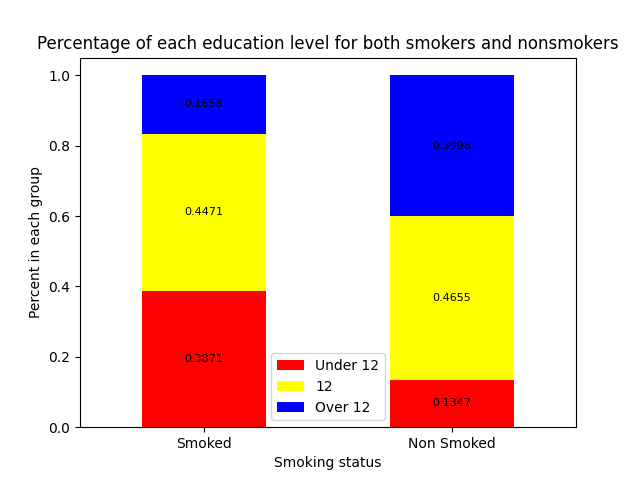
\includegraphics[scale=0.8]{10.png}
            \caption{Biểu đồ cột chồng thể hiện tỷ lệ về các cấp độ học vấn cho cả các bà mẹ hút thuốc và không hút thuốc trong thời gian thai kỳ trong nghiên cứu Missouri}
        \end{figure}

        \item Tạo một biểu đồ cột theo tuổi và tình trạng hút thuốc trong thời gian thai kỳ của các bà mẹ trong nghiên cứu Missouri (hình \ref{fig:Table1.16}).
        Trong từng nhóm, cột thể hiện tỷ lệ các bà mẹ hút thuốc trong nhóm.

        Ta thực hiện code vẽ biểu đồ cột thể hiện tỷ lệ các bà mẹ hút thuốc trong từng nhóm tuổi:

        \begin{python}
import numpy as np
import matplotlib.pyplot as plt

data = {"Under 18": 43, "18-19": 44, "20-24": 34, "25-29": 23, "30-34": 21, "Over 34": 26}

x = list(data.keys())
y = list(data.values())

fig, ax = plt.subplots(figsize=(9, 9))
ax.bar(x, y, color ="blue", width = 0.4)
plt.bar_label(ax.containers[0], label_type='edge', color='red', rotation=90, fontsize=15, padding=10)
 
plt.xlabel("Age group")
plt.ylabel("Percentage of mothers who smokes")
plt.title("Bar graph of age and smoking status")
plt.grid()
plt.show()
        \end{python}

        \begin{figure}[h!]
            \centering
            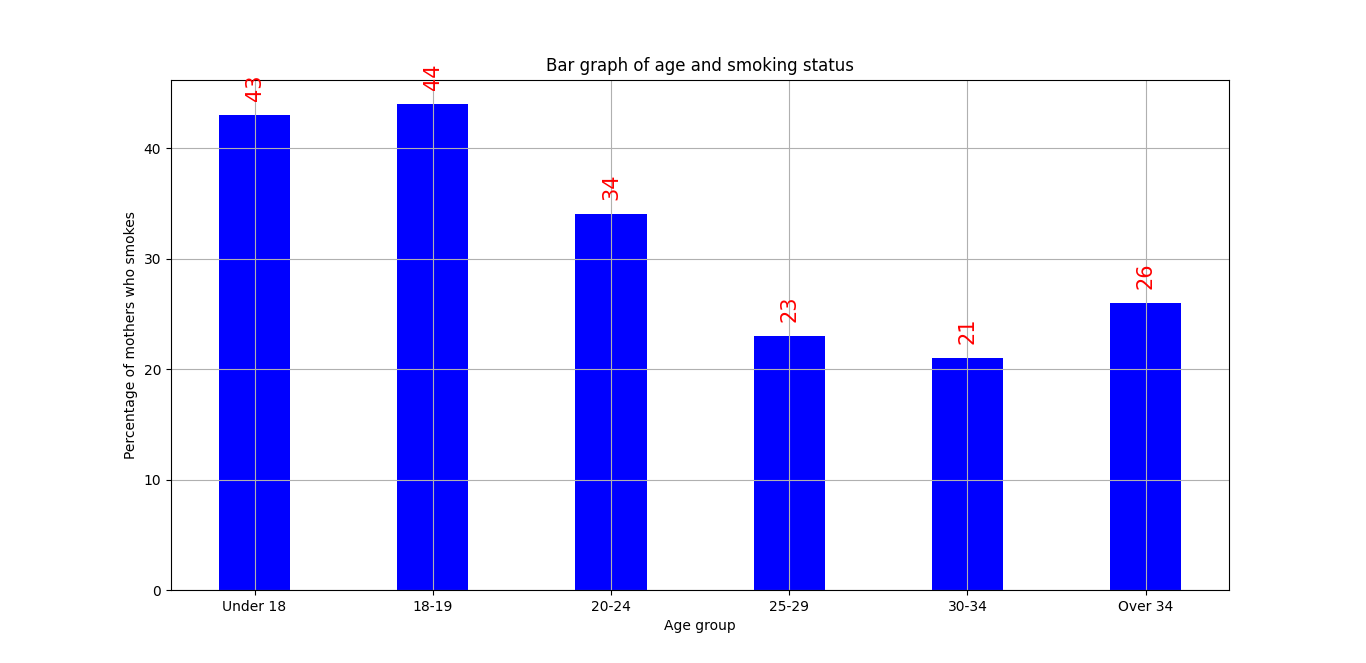
\includegraphics[scale=0.4]{11.png}
            \caption{Biểu đồ cột theo tuổi và tình trạng hút thuốc trong thời gian thai kỳ của các bà mẹ trong nghiên cứu Missouri}
        \end{figure}

        Ta tính độ tương quan giữa độ tuổi và tỷ lệ hút thuốc.

        Tuổi của người mẹ hoàn toàn có thể là yếu tố gây nhiễu giữa mối quan hệ giữa người mẹ có hút thuốc trong thời gian thai kỳ hay không và cân nặng khi sinh của em bé.
        Lý do vì tuổi của người mẹ có ảnh hưởng đến cân nặng của em bé, còn phụ nữ lớn tuổi có thể sinh những em bé có cân nặng thấp hơn.
        Mặt khác người mẹ trẻ tuổi có khả năng hút thuốc cao hơn và cũng có thể sinh ra em bé có cân nặng lớn hơn so với người mẹ đã có tuổi khá lớn.
        Điều này hoàn toàn có thể dẫn đến việc người mẹ hút thuốc trong thai kỳ làm có cân nặng em bé khi được sinh lớn hơn so với em bé được sinh bởi người mẹ không hút thuốc trong thai kỳ.

        \item Trong nghiên cứu Missouri, cân nặng trung bình khi sinh của các em bé mà có mẹ hút thuốc trong thời gian thai kỳ là 3180 grams và độ lệch chuẩn SD 500 grams.
        Cân nặng trung bình và độ lệch chuẩn SD trong đơn vị ounces. Biết rằng 0.0035 ounces tương đương 1 gram.

        Ta có cân nặng trung bình trong đơn vị ounces là: $3180\times 0.035=111.3$ (ounces) và độ lệch chuẩn SD trong đơn vị ounces là: $500 \times 0.035=17.5$ (ounces).
        
        \item Ta xét một danh sách các số $x_1, \dots, x_n$. Ta dịch và nhân từng số $x_i$ như sau:
        \begin{equation*}
            y_i = a + b x_i
        \end{equation*}

        Tìm trung bình và độ lệch chuẩn mới SD của danh sách $y_i, \dots, y_n$ được tính bằng trung bình và độ lệch chuẩn SD của danh sách ban đầu $x_1, \dots, x_n$.

        Ta tính $\bar{y}$:

        \begin{equation*}
            \begin{aligned}
                \bar{y} &= \sum_{i=1}^n \dfrac{y_i}{n} \\
                &= \sum_{i=1}^n \dfrac{a + b x_i}{n} \\
                &= \dfrac{na + b \sum_{i=1}^n x_i}{n} \\
                &= a + b \bar{x}
            \end{aligned}    
        \end{equation*}

        Ta tính $SD(y)$:

        \begin{equation*}
            \begin{aligned}
                SD(y) &= \sqrt{\dfrac{1}{n}\sum_{i=1}^n (y_i - \bar{y})^2} \\
                &= \sqrt{\dfrac{1}{n} \sum_{i=1}^n (a + b x_i - (a + b \bar{x})^2)} \\
                &= \sqrt{\dfrac{b^2}{n} \sum_{i=1}^n (x - x_i)^2} \\
                &= b \sqrt{\dfrac{1}{n}\sum_{i=1}^n (x - x_i)^2} \\
                &= b SD(x)
            \end{aligned}
        \end{equation*}

        Vậy ta có:

        \begin{equation*}
            \begin{cases}
                \bar{y} = a + b \bar{x} \\
                SD(y) = b SD(x)
            \end{cases}
        \end{equation*}

        \item Xét dữ liệu trong bài tập 13. Ta biểu diễn IQR của $y_1, \dots, y_n$ theo trung vị và IQR của $x_1, \dots, x_n$.
        Để đơn giản ta giả sử $y_1 < y_2 < \dots < y_n$ và giả sử $n$ là số lẻ.

        Ta nhận thấy $f(x) a + bx$ là hàm đơn điệu vì vậy vị trí của $Q_1(x), Q_2(x), Q_3 (x)$ cùng vị trí với $Q_1(y), Q_2(y), Q_3(y)$.
        Vì vậy ta có:

        \begin{equation*}
            \begin{cases}
                Q_1 (y) = a + bQ_1(x) \\
                Q_2 (y) = a + b Q_2(x) \\
                Q_3 (y) = a + b Q_3(x)
            \end{cases}
        \end{equation*}

        Vậy ta tính được:

        \begin{equation*}
            IQR(y) = Q_3 (y) - Q_1 (y) = a + b Q_3(x) - (a + b Q_1(x)) = b IQR(x)
        \end{equation*}

        \item Ta xét một danh sách các số $x_1, \dots, x_n$ với $x_1 < x_2 < \dots < x_n$, chứng minh rằng bằng cách thay $x_n$ bằng một số khác, trung bình và độ lệch chuẩn SD của danh sách có thể rất lớn.
        Nhưng điều này có đúng với trung vị và IQR? Giải thích.

        Ta nhận thấy khi thay $x_n$ bởi một số lớn thì trung vị (giá trị) chia danh sách làm hai nửa không bị ảnh hưởng.
        Và $Q_1, Q_3$ cũng không bị thay đổi dẫn đến $IQR = Q_3 - Q_1$ không thay đổi. 
        Vậy nên điều tương tự không đúng với trung vị và IQR.

        \item Ta giả sử có $n$ quan sát từ một phân phối chuẩn. Làm thế nào có thể sử dụng IQR của danh sách các quan sát để ước lượng $\sigma$?
        
        Như ở câu 8, ta đã biết được IQR của một phân phối chuẩn $\mathcal{N}(\mu, \sigma^2)$ là $IQR=1.349\sigma$.

        Ta sắp xếp lại danh sách theo thứ tự không giảm $x_1 \leq x_2 \leq \dots \leq x_n$.
        Từ $\bar{x}$, ta chọn hai điểm $Q_1$ là $x_k$ sao cho $k / n + 1 \approx 0.25$ và $Q_2$ là $x_j$ sao cho $j/ n+1 \approx 0.75$.
        Ta có thể ước lượng $\sigma$:

        \begin{equation*}
            \sigma = \dfrac{x_j - x_k}{1.349}
        \end{equation*}

        \item Ta giả sử phân vị mức $y_q$ của phân phối chuẩn $\mathcal{N}(\mu, \sigma^2)$ được vẽ theo phân vị mức $z_q$ của phân phối chuẩn tắc $\mathcal{N}(0, 1)$.
        Chứng minh rằng hệ số góc và hệ số chặn của đường thẳng là $\sigma$ và $\mu$ tương ứng.

        Ta có $Y \sim \mathcal{N}(\mu, \sigma^2)$ và $Z \sim \mathcal{N}(0, 1)$.
        \begin{equation*}
            \Phi(z_q) = P(Z < z_q) = q
        \end{equation*}

        Theo định nghĩa phân vị mức:
        \begin{equation*}
            P(Y < y_q) = P\Big(\dfrac{Y - \mu}{\sigma} < \dfrac{y_q - \mu}{\sigma}\Big) = \Phi\Big(\dfrac{y_q - \mu}{\sigma}\Big) = q
        \end{equation*}

        hay:

        \begin{equation*}
            \begin{aligned}
                \dfrac{y_q - \mu}{\sigma} &= z_q \\
                \Leftrightarrow y_q &= \mu + \sigma z_q
            \end{aligned}
        \end{equation*}

        Từ đây ta suy ra $y_q = \mu + \sigma z_q$ hay $y_q$ có thể được biểu diễn từ $z_q$ bằng phương trình đường thẳng với hệ số góc là $\sigma$ và hệ số chặn là $\mu$ (điều phải chứng minh).

        \item Ta giả sử $X_1, X_2, \dots, X_n$ tạo thành một mẫu từ phân phối chuẩn tắc.
        Chứng minh những điều sau:

        \begin{enumerate}
            \item $\Phi(X_1), \dots, \Phi(X_n)$ tương đương với lấy mẫu từ một phân phối đều trên $(0, 1)$
            
            Ta xét hai số $a$ và $b$ được lấy mẫu từ phân phối chuẩn tắc và $X \sim \mathcal{N}(0;1)$.
            Ta có:

            \begin{equation*}
                P(a < X < b) = \Phi(b) - \Phi(a)
            \end{equation*}

            Mặt khác, hai số $c, d \in (0, 1)$ và $Y \sim U \lbrack 0; 1 \rbrack$:

            \begin{equation*}
                P(c < Y < d) = d - c
            \end{equation*}

            Từ hai điều trên, ta nhận thấy $X_1, \dots, X_n$ được lấy mẫu từ phân bố chuẩn tắc thì tương đương $\Phi(X_1), \dots, \Phi(X_n)$ được lấy mẫu từ phân phối đều trên $(0,1)$.

            \item Đặt $U_1, \dots, U_n$ là một mẫu từ một phân phối chuẩn trên $(0, 1)$. Chứng minh:
            \begin{equation*}
                \mathbb{E} (U_{(k)}) = \dfrac{k}{n+1}
            \end{equation*}
            với $U_{(1)} \leq \dots \leq U_{(n)}$ là mẫu được sắp xếp theo thứ tự không giảm.
            
            Ta có hàm mật độ xác suất của phân phối đều trên đoạn $(0, 1)$ là:

            \begin{equation*}
                f(u) = \begin{cases}
                    1 \text{ nếu } 0 < u < 1 \\
                    0 \text{ nếu ngược lại}
                \end{cases}
            \end{equation*}

            Ta có hàm phân bố xác suất của phân phối đều trên đoạn $(0, 1)$ là:

            \begin{equation*}
                F(u) = \begin{cases}
                    0 \text{ nếu } u \leq 0 \\
                    u \text{ nếu } 0 < u < 1 \\
                    1 \text{ nếu } u \geq 1                    
                \end{cases}
            \end{equation*}

            Ta đặt $k$ là số nguyên sao cho $1 \leq k \leq n$.
            Xác suất để phần tử được sắp xếp thứ $k$ nhỏ hơn hoặc bằng một giá trị $u$ được cho bởi xác suất $k-1$ của $n$ quan sát nhỏ hơn $n$ và $n-k$ quan sát còn lại lớn hơn $u$.
            Ta tính xác suất $U_k \leq u$:

            \begin{equation*}
                P(U_k \leq u) = C_{k-1}^n u^{k-1} (1-u)^{n-k}
            \end{equation*}

            Ta tính hàm mật độ $f(u) = \dfrac{d P(U_k \leq u)}{du}$:

            \begin{equation*}
                f(u) = k C_k^n u^{k-1} (1-u)^{n-k}
            \end{equation*}

            Để tính $\mathbb{E}(U_{(k)})$, ta sử dụng công thức định nghĩa kỳ vọng:

            \begin{equation*}
                \begin{aligned}
                    \mathbb{E} (U_{(k)}) &= \int_{-\infty}^{\infty} u f(u) du = \int_{0}^{1} u f(u) du \\
                    &= \int_{0}^{1} k C_k^n u^k (1-u)^{n-k} du \\
                    &= k C_k^n  B(k+1, n-k+1) (\text{theo định nghĩa hàm beta } B(p, q) = \int_{0}^{1} x^{p-1}. (1-x)^{q-1}dx) \\
                    &= k C_k^n \dfrac{\Gamma(k+1)\Gamma(n-k+1)}{\Gamma(k+1 + (n-k+1))} (\text{liên hệ giữa hàm Beta và hàm Gamma } B(p, q) = \dfrac{\Gamma(p)\Gamma(q)}{\Gamma(p+q)}) \\
                    &= k C_k^n \dfrac{\Gamma(k+1)\Gamma(n-k+1)}{\Gamma(n+2)} \\
                    &= k C_k^n \dfrac{k! (n-k)!}{(n+1)!} (\text{theo công thức tính hàm Gamma } \Gamma(n)=(n-1)! \forall n \in \mathbb{N}) \\
                    &= k \dfrac{n!}{k!(n-k!)} \dfrac{k!(n-k)!}{(n+1)!} \\
                    &= \dfrac{k}{n+1}
                \end{aligned}
            \end{equation*}
        \end{enumerate}

        \item Chứng minh rằng trung bình $\bar{x}$ là hằng số cực tiểu hóa hàm sai lệch bình phương tương ứng với $c$:

        \begin{equation*}
            \sum_{i=1}^n (x_i - c)^2
        \end{equation*}

        Ta đặt $f(c) = \sum_{i=1}^n (x_i - c)^2$. Ta biến đổi:

        \begin{equation*}
            \begin{aligned}
                f(c) &= \sum_{i=1}^n (x_i - c)^2 \\
                &= \sum_{i=1}^n (x_i^2 - 2x_i c + c^2) \\
                &= \sum_{i=1}^n x_i^2 - 2(\sum_{i=1}^n x_i)c + n c^2 \\
                &= n\Bigg(c - \dfrac{\sum_{i=1}^n x_i}{n}\Bigg)^2 + \Bigg(\sum_{i=1}^n x_i^2 - \dfrac{(\sum_{i=1}^n x_i)^2}{n}\Bigg)
            \end{aligned}
        \end{equation*}

        Ta nhận thấy thành phần $\Bigg(\sum_{i=1}^n x_i^2 - \dfrac{(\sum_{i=1}^n x_i)^2}{n}\Bigg)$ không phụ thuộc vào $c$ vì vậy $f(c)$ nhỏ nhất khi $\Bigg(c - \dfrac{\sum_{i=1}^n x_i}{n}\Bigg)^2=0$ hay $c= \dfrac{\sum_{i=1}^n x_i}{n} = \bar{x}$ (điều phải chứng minh).

        \item Chứng minh rằng trung vị $\tilde{x}$ của $x_1, \dots, x_n$ là hằng số cực tiểu hóa sai lệch tuyệt đối tương ứng với $c$:

        \begin{equation*}
            \sum_{i=1}^n \lvert x_i - c \vert
        \end{equation*}

        Ta đặt $f(c) = \sum_{i=1}^n \lvert x_i - c \vert$
        Ta giả sử dãy $x_1, \dots, x_n$ được sắp xếp theo chiều không giảm hay $x_1 \leq x_2 \leq \dots \leq x_n$.
        Ta chọn một số $c$ sao cho $c < x_1$, khi đó:

        \begin{equation*}
            f(c) = \sum_{i=1}^n \lvert x_i - c \vert = \sum_{i=1}^n (x_i - c)
        \end{equation*}

        Nếu $c$ tăng dần nhưng vẫn nhỏ hơn $x_1$ thì từng thành phần $x_i - c$ sẽ giảm đến khi $c$ đạt đến $x_1$,
        vì vậy $f(x_1) < f(x) \thickspace \forall c < x_1$.
        Ta chọn một số $c$ sao cho $x_k \leq c \leq c + d \leq x_{k+1}(d > 0)$, khi đó:

        \begin{equation*}
            \begin{aligned}
                f(c + d) &= \sum_{i=1}^k (c + d - x_i) + \sum_{i=k+1}^n (x_i - (c + d)) \\
                &= dk + \sum_{i=1}^k (c - x_i) - d(n-k) + \sum_{i=k+1}^n (x_i - c) \\
                &= d(2k -n) + \sum_{i=1}^k (c - x_i) + \sum_{i=k+1}^n (x_i - c) \\
                &= d(2k - n) + f(c) \\
            \Rightarrow f(c + d) - f(c) &= d(2k - n)
            \end{aligned}
        \end{equation*}
        Ta nhận thấy khi $2k < n$, thì $f(c + d) < f(c)$, $2k = n$ thì $f(c+d)=f(c)$, $2k > n$ thì $f(c+d) > f(c)$.
        Hay khi $k$ tăng dần trước khi đạt đến $n/2$ thì f(c) giảm, và khi $k$ lớn hơn $n / 2$ thì f(c) tăng, nghĩa là f(c) sẽ đạt cực tiểu tại $k=n/2$ nghĩa là $k=n/2$ ở chính giữa dãy số đã được sắp xếp theo thứ tự không giảm.
        Vì vậy $f(c) = \sum_{i=1}^n \lvert x_i - c \vert$ đạt cực tiểu khi $c$ chính là trung vị của dãy $x_1, \dots, x_n$ (điều phải chứng minh).
    \end{enumerate}
\end{loigiai}

\newpage
\printbibliography[title={TÀI LIỆU THAM KHẢO}]

\end{document}